% $Id: ESMF_infradataoverview.tex,v 1.2 2003/10/25 03:07:39 cdeluca Exp $

\section{Overview of Infrastructure Data Classes}

{\tt Field} and {\tt Bundle} objects provide 
data access and data handling methods
in the Earth System Modeling Framework (ESMF).
They are the highest level objects in the
{\tt Gridded Component} object hierarchy.
Their methods are called both from user written
code as well as from other objects internal to the framework.

A {\tt Field} 
object encapsulates computational and/or observational data together 
with the underlying grid on which it is located.  
A {\tt Field} object provides the
application with both an overall logical view of the entire
dataset, as well as access to processor-local data after decomposition.
It provides methods for configuration, initialization, setting and
retrieving data values, data I/O, intercomponent data 
exchange, data regridding, and manipulation of attributes.

Groups of fields on the same underlying physical grid 
can be collected into a single
object called a {\tt Bundle}.  
A {\tt Bundle} provides two major functions: it allows groups of 
{\tt Fields}
to be manipulated using a single identifier, for example during
export or import of data between components; and it allows
data from multiple fields to be packed together in memory 
for higher locality of reference and ease in subsetting operations.
A {\tt Bundle} object contains methods
for setting and retrieving constituent fields, import and export
data exchange during intercomponent communication,
regridding, data I/O, and reordering of data in memory.


\subsection{Programming Model}

The following sections give a high level description of how
the overall application and components will operate,
focusing on how Fields and Bundles are created and used.
This is followed by a more detailed description of how
those functions are encapsulated into internal ESMF 
objects, followed by a detailed API (Application Programming
Interface) listing.

\subsection{Using Fields and Bundles}

\subsubsection{Field Initialization}

The following section describes issues related to
creation and initialization of Fields.

\begin{description}

\item{Application Initialization}
 
At Application initialization there is an opportunity to 
specify configuration attributes which can affect the
operation of Fields and Bundles.  The most likely used
attributes will control I/O specifications, e.g. 
filenames and file formats defaults.  These can be
queried at run time by the Field and Bundle code.

\item{Field Creation}

All versions of the {\tt ESMF\_FieldCreate} 
routines require a Grid object as input at some point.
The Grid contains the information needed to know which 
Decomposition Elements ({\tt DE}s) are participating in 
the processing of this Field.  

One of the Field decompositions
will have the responsibility for coordinating
any global operations on the Field (e.g. calls for Regridding,
Halo updates, I/O, etc).  It will communicate global information
to all the other Field decompositions.

Requests to access local Field data will not require 
communication overhead; the user code is expected to
query the Grid object to discover what part of the
overall dataset is local to this processor and do
computations based on that data.

The details of how the create process happens depends 
on which of the 
variants of the {\tt ESMF\_FieldCreate} call is used.
Some differences will be discussed below.

\item{Associating constructed data with Fields}

There are versions of the {\tt ESMF\_FieldCreate} interface
which allow user code to construct or read in data
outside of the ESMF and specify it either at Field create
time or add it to the Field later.  
In these cases, each DE must individually query the Grid object 
for details about what decomposition of the global grid is local 
to this PE so it correctly maps the local data decomposition
to the overall global Field.

The user code first calls 
{\tt ESMF\_ArrayCreateSpec} to create a
description of the data object (e.g. items are scalar or vector,
real or integer) and passes that into {\tt ESMF\_ArrayCreate}
to create an Array object.  That object can then be given
to the Field create code, with options to reference that array
or make a separate copy inside the Field. 

\item{Having Fields Allocate Space for Data}

There are versions of the {\tt ESMF\_FieldCreate} interface
which create the Field based on the input Grid.  The ESMF
can allocate the proper amount of 
space but not assign initial values.  The user code
can then detach the uninitialized buffer, set the
initial data values, and reattach the buffer.

\item{Field Read}

Fields can be created by the {\tt ESMF\_FieldRead}
routine, with options to create the Grid at this time
as well as creating the associated Arrays.
See the following section on Field I/O for a longer
discussion of Field Reads.

\end{description}

Fields can be created and destroyed
at any time during application execution.  However, the creation
and deletion of Fields requires interprocessor communication
and will require some time to complete.  It is not recommended
that Fields are created or destroyed
inside performance-critical computational loops.

Fields and Bundles are used in constructing 
the Import and Export states for component coupling, 
which requires that the 
Fields involved in data exchange be identified, as well as
which Transforms must be performed on them to make the
data compatible with the specifications of
receiving components.  

\subsubsection{Bundle Initialization}

It is not required that {\tt Bundles} be created or used.
{\tt Bundles} offer a way to group {\tt Fields} which share a
common {\tt Grid}, and optionally to pack the {\tt Field} data
together in a single buffer.

\begin{description}

\item{Bundle Creation from Existing Fields}

After creating multiple Fields, Bundles can be created
by calling the {\tt ESMF\_BundleCreate} subroutine.  There are
options to create a {\tt Bundle} which simply references
the data buffers of the existing {\tt Fields}, 
or the Bundle can make a separate copy of the data in a private 
Bundle data buffer.  If a data copy is made, there are options to
control the interleaving of the Field data in the Bundle data buffer.

All Fields in a bundle must share the same underlying Grid.
If the Bundle has a private data buffer, then the Fields must
all share a compatible mapping of data onto the Grid as well.

\end{description}

\subsubsection{Use During Execution}

Access to data is similar for {\tt Fields} and {\tt Bundles} with
packed data.  It is described below using the {\tt Field}
routines in the examples, but corresponding {\tt Bundle} level
routines exist.  To access data in a
Bundle which is not packed, the user must loop over the
Fields in the Bundles, querying for each
constituent Field and then using the Field level data interfaces.

\begin{description}

\item{Accessing Field Data}

The user code on each DE calls the {\tt ESMF\_FieldGridQuery}
routine to find out about the local subset of the data, including
the number of items, the extents
of the dimensions, and the corresponding coordinates of this
decomposition.

The user code can then call {\tt ESMF\_FieldDataDetach} to
begin iterating through the data.  This routine returns a
pointer to the buffer and marks the data as "in use by
the user code".  The ESMF cannot read or write that
data until {\tt ESMF\_FieldDataAttach} is called.  Once the data
is reattached the framework can use the data in regridding 
operations, halo updates, etc.  

If the user code only needs read-only access and wants
the option of greater concurrency, there is an option on the
Detach routine which says access will be read only.  There is
a corresponding {\tt ESMF\_FieldDataDrop} subroutine that must be called
after all access is done, but during this time other parts of
the code can also call {\tt ESMF\_FieldDataDetach} with the read-only
option so multiple readers are allowed.  However, if write access
is requested it will fail (or optionally, wait) until all readers 
are finished, and
then write access will be exclusive.   Requests for read access
will fail until the updated data is reattached. 
This does not, of course, preclude user code from passing around
buffer pointers directly and making whatever concurrent accesses to the
data buffer it wants.  These restrictions are only for internal
ESMF access.
(Note: This exclusive access may not be implemented if no user
code finds a need for it.)

There is a final data access option, {\tt ESMF\_FieldDataDetachCopy}
which returns a copy of the data buffer and does not mark the
Field data as detached or in use in any way.  The ESMF 
allocates space for this data buffer, so it becomes the
responsibility of the calling code to release that space 
when finished with it.

\end{description}


\subsubsection{Field and Bundle I/O}

The I/O component layer isolates the higher level Field
and Bundle
code from the details of format-dependent library calls
and some of the parallel I/O vs. scatter/gather issues, 
but the Field and Bundle code must specify 
what parts of the objects are read or written, and
whether to individual files or multiple files.  


\begin{description}

\item{Write}

The default behavior for Field and Bundle I/O
is to write the entire object into a single file,
preserving as much of the metadata information as is
possible with the selected I/O format.  This means
calling the appropriate Grid method to write the coordinates
into the file, and then calling an Array method to
write the associated data into the same file.  
Most formats have the concept of a variable or dataset;
the Field data will be written using the closest matching
concept for the format.  The coordinates and data will
be gathered for distributed fields so the contents can
be written as a unified whole.  These defaults can of
course be overridden by specifying the appropriate options.
Unless specified, the Field name will be used as the
variable or dataset name in the output file.
If attributes such as units are associated with the
Field they will be written as well.  

Since Bundles must share the same Grid, the Grid
will be written once into the file followed by the
data associated with each of the constituent Fields.
If the Bundle has an associated packed Array, the
default will still be to write the Field data as separate
variables in the file, but with an option to keep the
array packed and write it as a single variable in the file.
Other write options include writing each Field into a
separate file, duplicating the Grid in each file.

Other options include writing only the Grid or only the
Array, or writing each decomposition of the Field
or Bundle into separate files.

While it is expected that the I/O layer will isolate the
upper layers of code from most of the details of the
process, there are still some considerations at the
Field and Bundle level depending on 
where the data
is to be written from (single process or distributed) and into
how many files (single, multiple).
The following sections go into more detail about what the
the Field and Bundle objects needs to do in order to 
support various I/O strategies.

\begin{description}

\item{Serial write into a single file}

In this style, the data is gathered on a single PE
and written to a single file.  The Field code will have
to have gather calls which allow the data to be assembled
on a single processor for subsequent I/O layer calls.
There will be an asynchronous version of Write which
allows each PE to continue once it has sent its local
data decomposition to the PE where assembly is occurring.

\item{Parallel write into a single file}

The I/O layer will have to manage the gather.  In this
case each decomposition of the Field or Bundle makes
its own call to the I/O layer and assembly happens at
the lower layer.

\item{Parallel write into multiple files}

Each decomposition of the Field or Bundle makes its own
call to the I/O layer and writes only the local decomposition
of the Grid and Array.  One PE will have to
write out the Distributed Grid information so the parts can
be reconstituted into a single undecomposed object at 
the lower layer.

\item{Checkpoint/Restart considerations}

At some level the Checkpoint/Restart functions are
logically the same as Read/Write, and internally will use the
same I/O interfaces.  But by giving them different
names it is easy to separate out the places where performance
is more important than the format; the implication of calling
Checkpoint/Restart is that the data should be saved in the
most efficient method possible on this system.
The defaults for these routines will not match the defaults
for normal Read/Write.

\end{description}


\item{Read}

The defaults for Field and Bundle read will be to read
in any coordinate information and create a Grid, and then
any specified variables will be read and Fields created
for single variables, and Bundles for Fields which share
a Grid.  The defaults can be overridden by specifying
specific variables/datasets to read in, to read only the
data, only the grid, how to do the decomposition, and
other options which would normally be specified at 
Grid and Field and Bundle creation time.

Field and Bundle Read routines also have options to associate
an existing Grid with the Data in a file, so the Data is
read but the Grid is given as an input.

The input file formats vary in their capability to
carry enough metadata to allow the file to be read
in without directives from the calling code, but the
goal is to have the read default as much as is possible
to being controlled by the information in the file.

While most I/O options are encapsulated in the I/O layer,
the following section discusses some issues which pass
up above that layer.

\begin{description}

\item{Serial read from a single file}

The Field code may choose to first create an
undecomposed Field on a single PE and then invoke a
Field scatter routine which creates a Distributed Grid
and distributes subsets of the Array to different PEs.
The other option is to create a Physical and Distributed
Grid and then read in subsets in multiple calls to the
I/O layer and scatter pieces serially.  The former approach
is simpler but if the Field is too large to fit in the
physical memory of a single PE the latter approach may be
necessary.  For asychronous reads, the FieldRead call can
return immediately and a Poll routine must be available to
call later to see if the Field is ready.

\item{Parallel read from a single file}

The Field/Bundle code must first query for enough
Grid information to be able to construct a Distributed
Grid object which defines the mapping of decompositions
to the whole.  Then each individual PE can make calls
to the I/O layer to read the appropriate decomposition
into the local Array.  

\item{Parallel read from multiple files}

The Field/Bundle code must first query for enough
Grid information to be able to construct a Distributed
Grid object which defines the mapping of decompositions
to the whole.  Then each individual PE can make calls
to the I/O layer to read the appropriate decomposition
into the local Array.  

\item{Difficulties with Field Read}

Decompositions can vary from run to run; unless all data
is in a single file it is difficult to ensure that the data for
each decomposition is local to the correct processor.  This is
not a problem for Checkpoint/Restart during the run of a
single simulation, and a somewhat easier problem if restarting
a run with a different number of processors.  The restart files
can contain enough information to rebalance the data and get it
to the correct processors to continue.  But for data in an 
external data file format in multiple files, 
there may not be enough information about the original decomposition
to map the data correctly.

\end{description}

\end{description}

\subsubsection{Finalization}

\begin{description}

\item{Field Deletion}

There is a {\tt ESMF\_FieldDestroy} subroutine which releases
any data buffers which were allocated or copied by this Field,
and deletes the Field object.  Since the Grid can be shared
amongst multiple Fields, the Grid is not deleted by this call.

\item{Bundle Deletion}

If Bundles are used, the user must call the 
{\tt ESMF\_BundleDestroy} subroutine before deleting any constituent
Fields.  If a private Bundle data buffer exists, the space is
freed and all resources associated with the Bundle are released.
The constituent Fields are not deleted by this call, since they
can be contained by multiple Bundles.

\end{description}


\subsection{Internal Framework Use}

{\tt Fields} and {\tt Bundles} play a prominent role in {\tt Regrid} 
operations, in Halo updates,  
and in data exchanges between {\tt Components}.

\begin{description}

\item{Halo Updates from the Field's Perspective}

The Grid object manages Halo information such as how large the
halo area is around each Field, and what DEs contain the
corresponding Field.  There is an interface at the Field level
for initiating a Halo update, but the actual work happens
partly at the Field level (e.g. determining the data buffer is
attached and accessible by the ESMF, and accessing
the actual data values) and partly at the Distributed Grid
object level (e.g. determining the communication patterns, the
size and shape of the Halo region, etc).

\item{Field Import/Export between Components}

If a Field has been identified as being part of either the
Exchange Packet Import or Export process, then at the time
data is required the proper Transform subroutine must be 
called.  All Fields participating in the Transform must have
their data in the Attached state.  

\item{Field Export}

The Transform object contains
a series of functions which are called on the data.  The
original Field data is not altered; copies of the data are
created in the Export buffers and sent to the receiving
Components.  The decomposition of data from component to
component is expected to be different, so part of the transform
process is reshuffling the local Field data to match the
receiving component's Field decomposition.

\item{Field Import}

The Transform object contains a description of what data is
expected at Import time, and the data for the corresponding
Field objects are updated before the Import function returns.

\item{Regrid Operations}

The Regrid object contains methods for converting data from
one Grid to another, which may include interpolation, averaging,
or remapping operations.  The Regrid methods must be able to
first compute the map from the existing Grid, which it can
obtain by querying the Field, to the new Grid (specified by
the caller).  Then it must query the Field for how the data
is positioned on the existing Grid (cell centered, vertex, etc)
and how it is to be positioned on the new grid.  It then detaches
the data from the Field and does the necessary transformations
to construct a new Array.  It then can create the new field
with the new Grid and the new Array.  It then attaches
(or drops) the data from the existing Field to indicate it is
finished using it.

\item{Creating New Fields from a Combination of Existing Fields}

Creating new Fields from a weighted combination of existing
Fields is similar in procedure to Regridding, except that the
Grids are the same but the transformation of data is given 
by the caller.

\item{Changing Grids Underneath Fields}

The Grid object cannot be changed as long as it is being used
by any existing Fields.  To change the Grid object a copy of
the grid must be made and then new Fields created using the
new grid.  The Regrid functions are available if there's a 
mapping between the old Grid and the new one.

\item{Nested Grids and Fields}

The Regrid object understands about transformations between
grids, including mappings between Grids and nested Grids.

\end{description}

\newpage
\subsection{Object Model}

The following is a simplified UML diagram showing the relationships among
ESMF Field, Grid and Bundle classes.  See Appendix A, {\it A Brief 
Introduction to UML},
for a translation table that lists the symbols in the diagram and their 
meaning.

\begin{center}
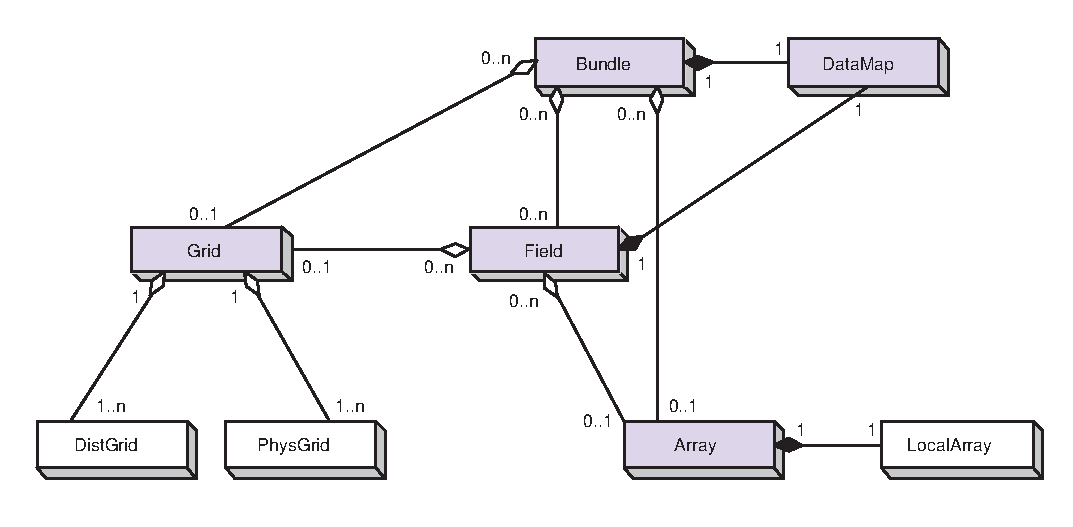
\includegraphics{Bundle_obj.eps}   
\end{center}

